%% LyX 2.3.6.1 created this file.  For more info, see http://www.lyx.org/.
%% Do not edit unless you really know what you are doing.
\documentclass[english]{article}
\usepackage[T1]{fontenc}
\usepackage[latin9]{inputenc}
\usepackage{float}

\makeatletter
%%%%%%%%%%%%%%%%%%%%%%%%%%%%%% User specified LaTeX commands.
% Header
\usepackage{fancyheadings}
\usepackage{amsmath}
\usepackage{amssymb}
\usepackage{graphicx}
\usepackage{booktabs}
\usepackage{tabularx}
\usepackage{lmodern}
\usepackage{outlines}
\usepackage{bm}
\usepackage{xr}
\usepackage{subfig}
\usepackage{algorithm,algpseudocode}
\usepackage{caption}
\usepackage{threeparttable}
\usepackage{multirow}
\usepackage{booktabs, tabularx}
\pagestyle{fancy}
\usepackage{pdflscape}
\usepackage{afterpage}
\usepackage{geometry}
\usepackage{color, colortbl}
\usepackage{xcolor}
\definecolor{maroon}{RGB}{139,0,0}
\definecolor{figray}{RGB}{128,128,128}
\definecolor{color1}{rgb}{0.5,0,0}    %The standard maroon
\definecolor{color2}{rgb}{0.65,0.65,0.65} %The lighter gray, not a standard color, darker that the usual light gray
\definecolor{color3}{rgb}{0.3,0.3,0.3}

\chead{}
\lhead{}
\rhead{\thepage}

\rfoot{}
\cfoot{}
\lfoot{}
\renewcommand{\headrulewidth}{0pt}

% Constants
\newcommand{\constp}[1]{\input{../assets/constants/#1.txt}\unskip}


% Section Header Styles
\usepackage{titlesec}
\titleformat*{\section}{\large\bfseries}
\titleformat*{\subsection}{\normalsize\bfseries}
\titleformat*{\subsubsection}{\normalsize\itshape}
\titleformat*{\paragraph}{\large\bfseries}
\titleformat*{\subparagraph}{\large\bfseries}

% Tikz Preamble entry
\usepackage{tikz}
\usepackage{tikz-network}
\usetikzlibrary{positioning}
\usetikzlibrary{arrows,decorations.pathmorphing,backgrounds,fit,positioning,shapes.symbols,chains}
\usetikzlibrary{math}
\usetikzlibrary{patterns}
\tikzset{>=latex}
\newcommand*\Texture[3][{\raisebox{0pt}[16pt][0pt]{ $+$}}]{\leavevmode\hbox to #2{\leaders\vbox to #3{\leaders\hbox{#1}\vfil}\hfil}}
\usetikzlibrary{fadings}
\usetikzlibrary{patterns}
\usepackage{pgfplots}
\pgfplotsset{compat=1.10}
\usepgfplotslibrary{fillbetween}
%

\makeatother

\usepackage{babel}
\begin{document}
\title{\vspace{-50pt}
}
\title{Dataset Documentation: Combining Human Expertise with Artificial Intelligence }
\author{Nikhil Agarwal, Alex Moehring, Pranav Rajpurkar, Tobias Salz\thanks{Agarwal: Department of Economics, MIT and NBER, email: agarwaln@mit.edu.
Moehring: MIT Sloan School of Management, email: moehring@mit.edu.
Rajpurkar: Department of Biomedical Informatics, Harvard Medical School,
email: pranav\_rajpurkar@hms.harvard.edu. Salz: Department of Economics,
MIT and NBER, email: tsalz@mit.edu. }}
\maketitle
\begin{abstract}
Artificial Intelligence (AI) is often perceived to supplant humans
in tasks requiring complex decision-making and reasoning. Contrary
to this view, this dataset provides experimental data on human-AI
collaboration to emphasize the need to study optimal collaboration
between human experts and AI tools. Using a self-designed interface,
we collected probabilistic assessments of \textasciitilde 280 radiologists
on a subset of 324 historical cases under different information and
sequence settings. This paper provides insight into the purpose, collection
approach and example uses of the dataset. The dataset was used to
study topics of how best to combine AI predictions with human input
informed by contextual information, and potential human biases in
using AI to inform decisions. With this resource, questions in healthcare
AI and decision-making can be explored. 
\end{abstract}

\section{Introduction}

The advances in AI have raised concerns of a potential displacement
of humans. While there is no doubt that AI has advanced enough to
perform tasks requiring complex reasoning, machines still cannot perform
the range of tasks that humans can {[}Andrew Ng{]}. In the context
of radiology, while deep learning has improved precision in image
recognition tasks, AI still cannot process clinical history information
the way humans can. This complementarity of AI's precision and humans'
contextual information necessitates the study of collaboration between
these two. 

With this purpose, we launched an experiment to collect chest X-ray
diagnostic assessments for retrospective patient cases of \textasciitilde 280
radiologists for 10 main thoracic pathologies (104 sub-pathologies
conditional on significant presence of main pathology) under different
information conditions and design tracks. We acquired these assessments
using a remote interface and through two modes: a) continuous probabilistic
value of pathology prevelance b) binarized recommendation on treatment/follow-up. 

In addition to that, the dataset contains information on time spent
by radiologist on cases, clinical history information of the patients
and values of two ground truth specifications defined by the researchers.
These ground truth variables derive from the assesessment of aggregating
the assessments of five board-certified radiologists at Mt. Sinai
hospital, and by estimating the leave-one-out mean of the probabilities
reported by the radiologists in the experiment. 

 Using this dataset one can answer questions like: 1. How do humans/radiologists
use AI assistance? 2. Is contextual information valuable? 3. Do the
costs of AI induced human biases outweigh the benefits? 4. What is
the trade-off, if any, between the cost savings on human effort and
decision-quality when delegating tasks to AI tools? 5. How do radiologists
with different skill levels use AI assistance? This is indicative
of the nature of research that can be undertaken with this data resource.
Existing literature on this topic compares the performance of AI
tools with human prediction power but does not explore how humans
collaborate with AI. This dataset aims to fill the gap in the AI-expert
collaboration field by providing experimental and quantitative assessment
of chest X-rays.

In the following sections we discuss the summary statistics, example
uses, variables, data collection and augmentation that gives the resulting
dataset. 

\section*{Dataset}

\subsection*{Data Collection}

The dataset was collected by researchers at Massachusetts Institute
of Technology (M.I.T.) and Harvard University using a remote interface
(Refer Appendix \ref{subsec:Appendix:-Experiment-Interface}). Participants
for this experiment were recruited from teleradiolgy companies (first
and third design) and the VinMac healthcare system in Vietnam(second
design). While all the participants were compensated for their participation
in the experiment, 

We used a designed three approaches to collect data on radiologists'
probabilities of chest X-ray interpretations to study human-AI collaboration
under various settings. These approaches were defined to mimic the
clinical setting for the participants. The proposed three hybrid designs
collect both within and across subject data. Within these designs,
the radiologists were randomized into different tracks depending on
the sequence of the following information environments:
\begin{enumerate}
    \item X-ray only
    \item X-ray with clinical history information
    \item X-ray with AI assistance 
    \item X-ray with AI assistance and clinical history information
\end{enumerate}
Along each track, every radiologist views one of the 324 historical
cases procured from the Stanford Healthcare System. These cases are
manually reviewed for public release and contain the X-ray and clinical
history information. We chose to use restrospective cases to limit
stakes in existing diagnostic procedures. For the AI assistance information
environment, we provide radiologists with CheXpert, developed by a
team of researchers at Stanford University. CheXpert, a deep learning
algorithm trained on 224,316 chest radiographs of 65,240 patients
uses only the X-ray image to predict the prevelance of fourteen thoracic
pathologies. 

Finally, to establish the ground truth for analyzing the quality of
the radiologists' assessment, aggregate data on the assessments of
five board-certified radiologists at Mt. Sinai hospital with at least
ten years of experience and chest radiology as a sub-specialty was
collected. 

\subsubsection*{Designs}

\subsubsection*{Design 1}

In this design, radiologists are assigned to a randomized sequence
track of the four information environments. They read fifteen patient
cases under every information environment in a sequential manner.
No case is read more than once. At the beginning of the experiment
every radiologist reads 8 practice cases. This design allows for both
within- and across-subject variation.
\begin{figure}[H]
\caption{Design 1\label{fig:Design-1}}
\begin{center}
\includegraphics[width=0.8\textwidth]{../../images/design1.pdf}
\end{center}
\end{figure}


\subsubsection*{Design 2}

In this design, radiologists diagnose sixty patient cases under the
four information environments. To ensure that radiologists do not
recall their/AI predictions from previous reads of the cases, a two-week
washout period is introduced between two experiment sessions. Within
every experiment session, fifteen patient cases are read under every
information environment in groups of five with no case repeated within
a session. The randomization occurs at the track-level where every
track has a different sequence of the information environments. 
\begin{figure}[H]
\caption{Design 2 \label{fig:Design-2}}
\begin{center}
\includegraphics[width=0.8\textwidth]{../../images/design2.pdf}
\end{center}
\end{figure}


\subsubsection*{Design 3}

In this design, radiologists diagnose fifty cases, first without and
then with AI assistance. Clinical history is randomly provided in
either the first or second half of images forming the basis of the
randomization. The cases diagnosed with and without clinical history
are different.
\begin{figure}[H]
\caption{Design 3 \label{fig:Design-3}}

\begin{center}
\includegraphics[width=0.8\textwidth]{../../images/design3.pdf}
\end{center}
\end{figure}


\subsection*{Structure 

Every observation in the dataset refers to a radiologist-patient-pathology
in a given experiment session. While there are no individual personal
identifiers in the dataset, we have defined unique identifiers for
each radiologist and patient-case used in the experiment. There is
also information on the design type and the sequence in which each
case was viewed by the radiologists within each experiment session.
Across different designs, the radiologists read cases under different
information environments. in which the case was read is also The major
variables of interest in this dataset are: probability, treat, alg\_pred
and the gt\_{*}{*} variables (refer to the variables list in Appendix
\ref{subsec:Appendix:-Variables}) that include information collected
using the remote interface. 

In radiology, a definitive ground truth is generally not available
because of inherent variability in radiologists and their image-reading
experience. In this dataset we introduce two important ground truth
measures: 1. Constructed by aggregating the probabilistic assessments
of five board-certified radiologists at Mt. Sinai Hospital. These
radiologists have at least ten years of experience with chest-radiology
as their sub-speciality. 2. Constructed using leave-one-out average
of radiologists' assessments from the experiment. The reads used to
calculate this ground truth were from the treatment arm with clinical
history but no AI assistance. Some other ground truth variables in
the dataset are: a. Continuous ground truth b. Ground truth constructed
using logodds ratio: $log\left[\frac{p}{1-p}\right]$. 


\subsection{Distribution and Maintenance}

\section{Preliminary Analysis}

The following sections intend to discuss possible uses of the dataset
for future research. 

\subsection{Summary Statistics}

In this section, we present some summary statistics on radiologists'
reported probability and decisions, their deviation from the defined
ground truth/AI, and the radiologist performance relative to AI. The
deviation variables are key to understanding radiologist accuracy
and AI influence in making diagnostic decisions. The values have been
reported across two pre-registered groups: a) Top-level with AI- This
includes the top-level pathologies of cardiomedistinal abnormality
and airspace opacity. b) Pooled with AI - This includes all the pathologies
with AI predictions excluding abnormality and support device hardware.
As shown in the table below, there is consistency in the reported
statistics across the different designs. 

\begin{table}[H]
\centering

\caption{Summary statistics\label{tab:summary_statistics}}

\newcommand{\probtoplevelexpmean}{$0.233$}
\newcommand{\probtoplevelexpsd}{$0.290$}
\newcommand{\probtoplevelexpobs}{$36,280$}
\newcommand{\followuptoplevelexpmean}{$0.322$}
\newcommand{\followuptoplevelexpsd}{$0.467$}
\newcommand{\followuptoplevelexpobs}{$36,280$}
\newcommand{\devgttoplevelexpmean}{$0.223$}
\newcommand{\devgttoplevelexpsd}{$0.281$}
\newcommand{\devgttoplevelexpobs}{$36,280$}
\newcommand{\devaitoplevelexpmean}{$0.191$}
\newcommand{\devaitoplevelexpsd}{$0.169$}
\newcommand{\devaitoplevelexpobs}{$36,280$}
\newcommand{\aiaccuracytoplevelexpmean}{$0.261$}
\newcommand{\aiaccuracytoplevelexpsd}{$0.195$}
\newcommand{\aiaccuracytoplevelexpobs}{$36,280$}
\newcommand{\cordectoplevelexpmean}{$0.695$}
\newcommand{\cordectoplevelexpsd}{$0.460$}
\newcommand{\cordectoplevelexpobs}{$36,280$}
\newcommand{\activetimetoplevelexpmean}{$2.82$}
\newcommand{\activetimetoplevelexpsd}{$2.63$}
\newcommand{\activetimetoplevelexpobs}{$36,270$}
\newcommand{\clickstoplevelexpmean}{$45$}
\newcommand{\clickstoplevelexpsd}{$33$}
\newcommand{\clickstoplevelexpobs}{$36,270$}
\newcommand{\probradexpmean}{$0.250$}
\newcommand{\probradexpsd}{$0.304$}
\newcommand{\probradexpobs}{$180$}
\newcommand{\followupradexpmean}{$0.333$}
\newcommand{\followupradexpsd}{$0.473$}
\newcommand{\followupradexpobs}{$180$}
\newcommand{\devgtradexpmean}{$0.276$}
\newcommand{\devgtradexpsd}{$0.323$}
\newcommand{\devgtradexpobs}{$180$}
\newcommand{\devairadexpmean}{$0.205$}
\newcommand{\devairadexpsd}{$0.179$}
\newcommand{\devairadexpobs}{$180$}
\newcommand{\aiaccuracyradexpmean}{$0.281$}
\newcommand{\aiaccuracyradexpsd}{$0.215$}
\newcommand{\aiaccuracyradexpobs}{$180$}
\newcommand{\cordecradexpmean}{$0.678$}
\newcommand{\cordecradexpsd}{$0.469$}
\newcommand{\cordecradexpobs}{$180$}
\newcommand{\activetimeradexpmean}{$3.19$}
\newcommand{\activetimeradexpsd}{$3.24$}
\newcommand{\activetimeradexpobs}{$180$}
\newcommand{\clicksradexpmean}{$48$}
\newcommand{\clicksradexpsd}{$35$}
\newcommand{\clicksradexpobs}{$180$}
\newcommand{\probpooledaiexpmean}{$0.083$}
\newcommand{\probpooledaiexpsd}{$0.201$}
\newcommand{\probpooledaiexpobs}{$235,820$}
\newcommand{\followuppooledaiexpmean}{$0.122$}
\newcommand{\followuppooledaiexpsd}{$0.328$}
\newcommand{\followuppooledaiexpobs}{$235,820$}
\newcommand{\devgtpooledaiexpmean}{$0.085$}
\newcommand{\devgtpooledaiexpsd}{$0.205$}
\newcommand{\devgtpooledaiexpobs}{$235,820$}
\newcommand{\devaipooledaiexpmean}{$0.100$}
\newcommand{\devaipooledaiexpsd}{$0.135$}
\newcommand{\devaipooledaiexpobs}{$235,820$}
\newcommand{\aiaccuracypooledaiexpmean}{$0.117$}
\newcommand{\aiaccuracypooledaiexpsd}{$0.156$}
\newcommand{\aiaccuracypooledaiexpobs}{$235,820$}
\newcommand{\cordecpooledaiexpmean}{$0.882$}
\newcommand{\cordecpooledaiexpsd}{$0.323$}
\newcommand{\cordecpooledaiexpobs}{$235,820$}
\newcommand{\activetimepooledaiexpmean}{$2.82$}
\newcommand{\activetimepooledaiexpsd}{$2.63$}
\newcommand{\activetimepooledaiexpobs}{$235,755$}
\newcommand{\clickspooledaiexpmean}{$45$}
\newcommand{\clickspooledaiexpsd}{$33$}
\newcommand{\clickspooledaiexpobs}{$235,755$}
\newcommand{\probnormalexpmean}{$0.540$}
\newcommand{\probnormalexpsd}{$0.329$}
\newcommand{\probnormalexpobs}{$18,140$}
\newcommand{\followupnormalexpmean}{$0.528$}
\newcommand{\followupnormalexpsd}{$0.499$}
\newcommand{\followupnormalexpobs}{$18,140$}
\newcommand{\devgtnormalexpmean}{$0.423$}
\newcommand{\devgtnormalexpsd}{$0.323$}
\newcommand{\devgtnormalexpobs}{$18,140$}
\newcommand{\devainormalexpmean}{$0.245$}
\newcommand{\devainormalexpsd}{$0.204$}
\newcommand{\devainormalexpobs}{$18,140$}
\newcommand{\aiaccuracynormalexpmean}{$0.561$}
\newcommand{\aiaccuracynormalexpsd}{$0.279$}
\newcommand{\aiaccuracynormalexpobs}{$18,140$}
\newcommand{\cordecnormalexpmean}{$0.532$}
\newcommand{\cordecnormalexpsd}{$0.499$}
\newcommand{\cordecnormalexpobs}{$18,140$}
\newcommand{\activetimenormalexpmean}{$2.82$}
\newcommand{\activetimenormalexpsd}{$2.63$}
\newcommand{\activetimenormalexpobs}{$18,135$}
\newcommand{\clicksnormalexpmean}{$45$}
\newcommand{\clicksnormalexpsd}{$33$}
\newcommand{\clicksnormalexpobs}{$18,135$}
\newcommand{\probpooledexpmean}{$0.031$}
\newcommand{\probpooledexpsd}{$0.132$}
\newcommand{\probpooledexpobs}{$1,850,280$}
\newcommand{\followuppooledexpmean}{$0.077$}
\newcommand{\followuppooledexpsd}{$0.266$}
\newcommand{\followuppooledexpobs}{$526,060$}
\newcommand{\devgtpooledexpmean}{$0.032$}
\newcommand{\devgtpooledexpsd}{$0.133$}
\newcommand{\devgtpooledexpobs}{$1,850,280$}
\newcommand{\devaipooledexpmean}{$0.100$}
\newcommand{\devaipooledexpsd}{$0.135$}
\newcommand{\devaipooledexpobs}{$235,820$}
\newcommand{\aiaccuracypooledexpmean}{$0.117$}
\newcommand{\aiaccuracypooledexpsd}{$0.156$}
\newcommand{\aiaccuracypooledexpobs}{$235,820$}
\newcommand{\cordecpooledexpmean}{$0.979$}
\newcommand{\cordecpooledexpsd}{$0.144$}
\newcommand{\cordecpooledexpobs}{$1,850,280$}
\newcommand{\activetimepooledexpmean}{$2.82$}
\newcommand{\activetimepooledexpsd}{$2.63$}
\newcommand{\activetimepooledexpobs}{$1,849,770$}
\newcommand{\clickspooledexpmean}{$45$}
\newcommand{\clickspooledexpsd}{$33$}
\newcommand{\clickspooledexpobs}{$1,849,770$}

\newcommand{\probtopleveldomean}{$0.214$}
\newcommand{\probtopleveldosd}{$0.287$}
\newcommand{\probtopleveldoobs}{$13,440$}
\newcommand{\followuptopleveldomean}{$0.277$}
\newcommand{\followuptopleveldosd}{$0.448$}
\newcommand{\followuptopleveldoobs}{$13,440$}
\newcommand{\devgttopleveldomean}{$0.218$}
\newcommand{\devgttopleveldosd}{$0.290$}
\newcommand{\devgttopleveldoobs}{$13,440$}
\newcommand{\devaitopleveldomean}{$0.201$}
\newcommand{\devaitopleveldosd}{$0.171$}
\newcommand{\devaitopleveldoobs}{$13,440$}
\newcommand{\aiaccuracytopleveldomean}{$0.260$}
\newcommand{\aiaccuracytopleveldosd}{$0.193$}
\newcommand{\aiaccuracytopleveldoobs}{$13,440$}
\newcommand{\cordectopleveldomean}{$0.736$}
\newcommand{\cordectopleveldosd}{$0.441$}
\newcommand{\cordectopleveldoobs}{$13,440$}
\newcommand{\activetimetopleveldomean}{$3.03$}
\newcommand{\activetimetopleveldosd}{$3.17$}
\newcommand{\activetimetopleveldoobs}{$13,436$}
\newcommand{\clickstopleveldomean}{$43$}
\newcommand{\clickstopleveldosd}{$32$}
\newcommand{\clickstopleveldoobs}{$13,436$}
\newcommand{\probraddomean}{$0.180$}
\newcommand{\probraddosd}{$0.282$}
\newcommand{\probraddoobs}{$112$}
\newcommand{\followupraddomean}{$0.196$}
\newcommand{\followupraddosd}{$0.399$}
\newcommand{\followupraddoobs}{$112$}
\newcommand{\devgtraddomean}{$0.192$}
\newcommand{\devgtraddosd}{$0.295$}
\newcommand{\devgtraddoobs}{$112$}
\newcommand{\devairaddomean}{$0.174$}
\newcommand{\devairaddosd}{$0.164$}
\newcommand{\devairaddoobs}{$112$}
\newcommand{\aiaccuracyraddomean}{$0.234$}
\newcommand{\aiaccuracyraddosd}{$0.192$}
\newcommand{\aiaccuracyraddoobs}{$112$}
\newcommand{\cordecraddomean}{$0.830$}
\newcommand{\cordecraddosd}{$0.377$}
\newcommand{\cordecraddoobs}{$112$}
\newcommand{\activetimeraddomean}{$2.83$}
\newcommand{\activetimeraddosd}{$2.57$}
\newcommand{\activetimeraddoobs}{$112$}
\newcommand{\clicksraddomean}{$39$}
\newcommand{\clicksraddosd}{$26$}
\newcommand{\clicksraddoobs}{$112$}
\newcommand{\probpooledaidomean}{$0.074$}
\newcommand{\probpooledaidosd}{$0.194$}
\newcommand{\probpooledaidoobs}{$87,360$}
\newcommand{\followuppooledaidomean}{$0.101$}
\newcommand{\followuppooledaidosd}{$0.302$}
\newcommand{\followuppooledaidoobs}{$87,360$}
\newcommand{\devgtpooledaidomean}{$0.079$}
\newcommand{\devgtpooledaidosd}{$0.206$}
\newcommand{\devgtpooledaidoobs}{$87,360$}
\newcommand{\devaipooledaidomean}{$0.104$}
\newcommand{\devaipooledaidosd}{$0.137$}
\newcommand{\devaipooledaidoobs}{$87,360$}
\newcommand{\aiaccuracypooledaidomean}{$0.117$}
\newcommand{\aiaccuracypooledaidosd}{$0.155$}
\newcommand{\aiaccuracypooledaidoobs}{$87,360$}
\newcommand{\cordecpooledaidomean}{$0.901$}
\newcommand{\cordecpooledaidosd}{$0.299$}
\newcommand{\cordecpooledaidoobs}{$87,360$}
\newcommand{\activetimepooledaidomean}{$3.03$}
\newcommand{\activetimepooledaidosd}{$3.17$}
\newcommand{\activetimepooledaidoobs}{$87,334$}
\newcommand{\clickspooledaidomean}{$43$}
\newcommand{\clickspooledaidosd}{$32$}
\newcommand{\clickspooledaidoobs}{$87,334$}
\newcommand{\probnormaldomean}{$0.495$}
\newcommand{\probnormaldosd}{$0.324$}
\newcommand{\probnormaldoobs}{$6,720$}
\newcommand{\followupnormaldomean}{$0.526$}
\newcommand{\followupnormaldosd}{$0.499$}
\newcommand{\followupnormaldoobs}{$6,720$}
\newcommand{\devgtnormaldomean}{$0.400$}
\newcommand{\devgtnormaldosd}{$0.308$}
\newcommand{\devgtnormaldoobs}{$6,720$}
\newcommand{\devainormaldomean}{$0.277$}
\newcommand{\devainormaldosd}{$0.211$}
\newcommand{\devainormaldoobs}{$6,720$}
\newcommand{\aiaccuracynormaldomean}{$0.565$}
\newcommand{\aiaccuracynormaldosd}{$0.279$}
\newcommand{\aiaccuracynormaldoobs}{$6,720$}
\newcommand{\cordecnormaldomean}{$0.534$}
\newcommand{\cordecnormaldosd}{$0.499$}
\newcommand{\cordecnormaldoobs}{$6,720$}
\newcommand{\activetimenormaldomean}{$3.03$}
\newcommand{\activetimenormaldosd}{$3.17$}
\newcommand{\activetimenormaldoobs}{$6,718$}
\newcommand{\clicksnormaldomean}{$43$}
\newcommand{\clicksnormaldosd}{$32$}
\newcommand{\clicksnormaldoobs}{$6,718$}
\newcommand{\probpooleddomean}{$0.029$}
\newcommand{\probpooleddosd}{$0.127$}
\newcommand{\probpooleddoobs}{$685,440$}
\newcommand{\followuppooleddomean}{$0.066$}
\newcommand{\followuppooleddosd}{$0.247$}
\newcommand{\followuppooleddoobs}{$194,880$}
\newcommand{\devgtpooleddomean}{$0.030$}
\newcommand{\devgtpooleddosd}{$0.134$}
\newcommand{\devgtpooleddoobs}{$685,440$}
\newcommand{\devaipooleddomean}{$0.104$}
\newcommand{\devaipooleddosd}{$0.137$}
\newcommand{\devaipooleddoobs}{$87,360$}
\newcommand{\aiaccuracypooleddomean}{$0.117$}
\newcommand{\aiaccuracypooleddosd}{$0.155$}
\newcommand{\aiaccuracypooleddoobs}{$87,360$}
\newcommand{\cordecpooleddomean}{$0.982$}
\newcommand{\cordecpooleddosd}{$0.134$}
\newcommand{\cordecpooleddoobs}{$685,440$}
\newcommand{\activetimepooleddomean}{$3.03$}
\newcommand{\activetimepooleddosd}{$3.17$}
\newcommand{\activetimepooleddoobs}{$685,236$}
\newcommand{\clickspooleddomean}{$43$}
\newcommand{\clickspooleddosd}{$32$}
\newcommand{\clickspooleddoobs}{$685,236$}

\newcommand{\probtopleveltwmean}{$0.245$}
\newcommand{\probtopleveltwsd}{$0.278$}
\newcommand{\probtopleveltwobs}{$15,840$}
\newcommand{\followuptopleveltwmean}{$0.400$}
\newcommand{\followuptopleveltwsd}{$0.490$}
\newcommand{\followuptopleveltwobs}{$15,840$}
\newcommand{\devgttopleveltwmean}{$0.232$}
\newcommand{\devgttopleveltwsd}{$0.265$}
\newcommand{\devgttopleveltwobs}{$15,840$}
\newcommand{\devaitopleveltwmean}{$0.172$}
\newcommand{\devaitopleveltwsd}{$0.159$}
\newcommand{\devaitopleveltwobs}{$15,840$}
\newcommand{\aiaccuracytopleveltwmean}{$0.261$}
\newcommand{\aiaccuracytopleveltwsd}{$0.195$}
\newcommand{\aiaccuracytopleveltwobs}{$15,840$}
\newcommand{\cordectopleveltwmean}{$0.620$}
\newcommand{\cordectopleveltwsd}{$0.485$}
\newcommand{\cordectopleveltwobs}{$15,840$}
\newcommand{\activetimetopleveltwmean}{$2.76$}
\newcommand{\activetimetopleveltwsd}{$1.93$}
\newcommand{\activetimetopleveltwobs}{$15,834$}
\newcommand{\clickstopleveltwmean}{$49$}
\newcommand{\clickstopleveltwsd}{$30$}
\newcommand{\clickstopleveltwobs}{$15,834$}
\newcommand{\probradtwmean}{$0.188$}
\newcommand{\probradtwsd}{$0.261$}
\newcommand{\probradtwobs}{$33$}
\newcommand{\followupradtwmean}{$0.333$}
\newcommand{\followupradtwsd}{$0.479$}
\newcommand{\followupradtwobs}{$33$}
\newcommand{\devgtradtwmean}{$0.141$}
\newcommand{\devgtradtwsd}{$0.190$}
\newcommand{\devgtradtwobs}{$33$}
\newcommand{\devairadtwmean}{$0.138$}
\newcommand{\devairadtwsd}{$0.131$}
\newcommand{\devairadtwobs}{$33$}
\newcommand{\aiaccuracyradtwmean}{$0.214$}
\newcommand{\aiaccuracyradtwsd}{$0.152$}
\newcommand{\aiaccuracyradtwobs}{$33$}
\newcommand{\cordecradtwmean}{$0.758$}
\newcommand{\cordecradtwsd}{$0.435$}
\newcommand{\cordecradtwobs}{$33$}
\newcommand{\activetimeradtwmean}{$2.33$}
\newcommand{\activetimeradtwsd}{$1.32$}
\newcommand{\activetimeradtwobs}{$33$}
\newcommand{\clicksradtwmean}{$42$}
\newcommand{\clicksradtwsd}{$21$}
\newcommand{\clicksradtwobs}{$33$}
\newcommand{\probpooledaitwmean}{$0.090$}
\newcommand{\probpooledaitwsd}{$0.199$}
\newcommand{\probpooledaitwobs}{$102,960$}
\newcommand{\followuppooledaitwmean}{$0.154$}
\newcommand{\followuppooledaitwsd}{$0.361$}
\newcommand{\followuppooledaitwobs}{$102,960$}
\newcommand{\devgtpooledaitwmean}{$0.090$}
\newcommand{\devgtpooledaitwsd}{$0.199$}
\newcommand{\devgtpooledaitwobs}{$102,960$}
\newcommand{\devaipooledaitwmean}{$0.094$}
\newcommand{\devaipooledaitwsd}{$0.127$}
\newcommand{\devaipooledaitwobs}{$102,960$}
\newcommand{\aiaccuracypooledaitwmean}{$0.117$}
\newcommand{\aiaccuracypooledaitwsd}{$0.156$}
\newcommand{\aiaccuracypooledaitwobs}{$102,960$}
\newcommand{\cordecpooledaitwmean}{$0.853$}
\newcommand{\cordecpooledaitwsd}{$0.354$}
\newcommand{\cordecpooledaitwobs}{$102,960$}
\newcommand{\activetimepooledaitwmean}{$2.76$}
\newcommand{\activetimepooledaitwsd}{$1.93$}
\newcommand{\activetimepooledaitwobs}{$102,921$}
\newcommand{\clickspooledaitwmean}{$49$}
\newcommand{\clickspooledaitwsd}{$30$}
\newcommand{\clickspooledaitwobs}{$102,921$}
\newcommand{\probnormaltwmean}{$0.603$}
\newcommand{\probnormaltwsd}{$0.310$}
\newcommand{\probnormaltwobs}{$7,920$}
\newcommand{\followupnormaltwmean}{$0.566$}
\newcommand{\followupnormaltwsd}{$0.496$}
\newcommand{\followupnormaltwobs}{$7,920$}
\newcommand{\devgtnormaltwmean}{$0.464$}
\newcommand{\devgtnormaltwsd}{$0.325$}
\newcommand{\devgtnormaltwobs}{$7,920$}
\newcommand{\devainormaltwmean}{$0.195$}
\newcommand{\devainormaltwsd}{$0.174$}
\newcommand{\devainormaltwobs}{$7,920$}
\newcommand{\aiaccuracynormaltwmean}{$0.559$}
\newcommand{\aiaccuracynormaltwsd}{$0.280$}
\newcommand{\aiaccuracynormaltwobs}{$7,920$}
\newcommand{\cordecnormaltwmean}{$0.487$}
\newcommand{\cordecnormaltwsd}{$0.500$}
\newcommand{\cordecnormaltwobs}{$7,920$}
\newcommand{\activetimenormaltwmean}{$2.76$}
\newcommand{\activetimenormaltwsd}{$1.93$}
\newcommand{\activetimenormaltwobs}{$7,917$}
\newcommand{\clicksnormaltwmean}{$49$}
\newcommand{\clicksnormaltwsd}{$30$}
\newcommand{\clicksnormaltwobs}{$7,917$}
\newcommand{\probpooledtwmean}{$0.034$}
\newcommand{\probpooledtwsd}{$0.132$}
\newcommand{\probpooledtwobs}{$807,840$}
\newcommand{\followuppooledtwmean}{$0.096$}
\newcommand{\followuppooledtwsd}{$0.294$}
\newcommand{\followuppooledtwobs}{$229,680$}
\newcommand{\devgtpooledtwmean}{$0.034$}
\newcommand{\devgtpooledtwsd}{$0.130$}
\newcommand{\devgtpooledtwobs}{$807,840$}
\newcommand{\devaipooledtwmean}{$0.094$}
\newcommand{\devaipooledtwsd}{$0.127$}
\newcommand{\devaipooledtwobs}{$102,960$}
\newcommand{\aiaccuracypooledtwmean}{$0.117$}
\newcommand{\aiaccuracypooledtwsd}{$0.156$}
\newcommand{\aiaccuracypooledtwobs}{$102,960$}
\newcommand{\cordecpooledtwmean}{$0.974$}
\newcommand{\cordecpooledtwsd}{$0.160$}
\newcommand{\cordecpooledtwobs}{$807,840$}
\newcommand{\activetimepooledtwmean}{$2.76$}
\newcommand{\activetimepooledtwsd}{$1.93$}
\newcommand{\activetimepooledtwobs}{$807,534$}
\newcommand{\clickspooledtwmean}{$49$}
\newcommand{\clickspooledtwsd}{$30$}
\newcommand{\clickspooledtwobs}{$807,534$}

\newcommand{\probtoplevelthmean}{$0.240$}
\newcommand{\probtoplevelthsd}{$0.322$}
\newcommand{\probtoplevelthobs}{$7,000$}
\newcommand{\followuptoplevelthmean}{$0.231$}
\newcommand{\followuptoplevelthsd}{$0.421$}
\newcommand{\followuptoplevelthobs}{$7,000$}
\newcommand{\devgttoplevelthmean}{$0.212$}
\newcommand{\devgttoplevelthsd}{$0.297$}
\newcommand{\devgttoplevelthobs}{$7,000$}
\newcommand{\devaitoplevelthmean}{$0.216$}
\newcommand{\devaitoplevelthsd}{$0.182$}
\newcommand{\devaitoplevelthobs}{$7,000$}
\newcommand{\aiaccuracytoplevelthmean}{$0.260$}
\newcommand{\aiaccuracytoplevelthsd}{$0.196$}
\newcommand{\aiaccuracytoplevelthobs}{$7,000$}
\newcommand{\cordectoplevelthmean}{$0.785$}
\newcommand{\cordectoplevelthsd}{$0.411$}
\newcommand{\cordectoplevelthobs}{$7,000$}
\newcommand{\activetimetoplevelthmean}{$2.58$}
\newcommand{\activetimetoplevelthsd}{$2.80$}
\newcommand{\activetimetoplevelthobs}{$7,000$}
\newcommand{\clickstoplevelthmean}{$42$}
\newcommand{\clickstoplevelthsd}{$39$}
\newcommand{\clickstoplevelthobs}{$7,000$}
\newcommand{\probradthmean}{$0.232$}
\newcommand{\probradthsd}{$0.319$}
\newcommand{\probradthobs}{$35$}
\newcommand{\followupradthmean}{$0.200$}
\newcommand{\followupradthsd}{$0.406$}
\newcommand{\followupradthobs}{$35$}
\newcommand{\devgtradthmean}{$0.150$}
\newcommand{\devgtradthsd}{$0.223$}
\newcommand{\devgtradthobs}{$35$}
\newcommand{\devairadthmean}{$0.212$}
\newcommand{\devairadthsd}{$0.180$}
\newcommand{\devairadthobs}{$35$}
\newcommand{\aiaccuracyradthmean}{$0.258$}
\newcommand{\aiaccuracyradthsd}{$0.193$}
\newcommand{\aiaccuracyradthobs}{$35$}
\newcommand{\cordecradthmean}{$0.829$}
\newcommand{\cordecradthsd}{$0.382$}
\newcommand{\cordecradthobs}{$35$}
\newcommand{\activetimeradthmean}{$2.52$}
\newcommand{\activetimeradthsd}{$2.53$}
\newcommand{\activetimeradthobs}{$35$}
\newcommand{\clicksradthmean}{$41$}
\newcommand{\clicksradthsd}{$33$}
\newcommand{\clicksradthobs}{$35$}
\newcommand{\probpooledaithmean}{$0.085$}
\newcommand{\probpooledaithsd}{$0.218$}
\newcommand{\probpooledaithobs}{$45,500$}
\newcommand{\followuppooledaithmean}{$0.092$}
\newcommand{\followuppooledaithsd}{$0.289$}
\newcommand{\followuppooledaithobs}{$45,500$}
\newcommand{\devgtpooledaithmean}{$0.083$}
\newcommand{\devgtpooledaithsd}{$0.215$}
\newcommand{\devgtpooledaithobs}{$45,500$}
\newcommand{\devaipooledaithmean}{$0.110$}
\newcommand{\devaipooledaithsd}{$0.147$}
\newcommand{\devaipooledaithobs}{$45,500$}
\newcommand{\aiaccuracypooledaithmean}{$0.117$}
\newcommand{\aiaccuracypooledaithsd}{$0.156$}
\newcommand{\aiaccuracypooledaithobs}{$45,500$}
\newcommand{\cordecpooledaithmean}{$0.911$}
\newcommand{\cordecpooledaithsd}{$0.284$}
\newcommand{\cordecpooledaithobs}{$45,500$}
\newcommand{\activetimepooledaithmean}{$2.58$}
\newcommand{\activetimepooledaithsd}{$2.80$}
\newcommand{\activetimepooledaithobs}{$45,500$}
\newcommand{\clickspooledaithmean}{$42$}
\newcommand{\clickspooledaithsd}{$39$}
\newcommand{\clickspooledaithobs}{$45,500$}
\newcommand{\probnormalthmean}{$0.484$}
\newcommand{\probnormalthsd}{$0.356$}
\newcommand{\probnormalthobs}{$3,500$}
\newcommand{\followupnormalthmean}{$0.445$}
\newcommand{\followupnormalthsd}{$0.497$}
\newcommand{\followupnormalthobs}{$3,500$}
\newcommand{\devgtnormalthmean}{$0.372$}
\newcommand{\devgtnormalthsd}{$0.333$}
\newcommand{\devgtnormalthobs}{$3,500$}
\newcommand{\devainormalthmean}{$0.298$}
\newcommand{\devainormalthsd}{$0.226$}
\newcommand{\devainormalthobs}{$3,500$}
\newcommand{\aiaccuracynormalthmean}{$0.559$}
\newcommand{\aiaccuracynormalthsd}{$0.279$}
\newcommand{\aiaccuracynormalthobs}{$3,500$}
\newcommand{\cordecnormalthmean}{$0.630$}
\newcommand{\cordecnormalthsd}{$0.483$}
\newcommand{\cordecnormalthobs}{$3,500$}
\newcommand{\activetimenormalthmean}{$2.58$}
\newcommand{\activetimenormalthsd}{$2.80$}
\newcommand{\activetimenormalthobs}{$3,500$}
\newcommand{\clicksnormalthmean}{$42$}
\newcommand{\clicksnormalthsd}{$39$}
\newcommand{\clicksnormalthobs}{$3,500$}
\newcommand{\probpooledthmean}{$0.031$}
\newcommand{\probpooledthsd}{$0.141$}
\newcommand{\probpooledthobs}{$357,000$}
\newcommand{\followuppooledthmean}{$0.054$}
\newcommand{\followuppooledthsd}{$0.226$}
\newcommand{\followuppooledthobs}{$101,500$}
\newcommand{\devgtpooledthmean}{$0.030$}
\newcommand{\devgtpooledthsd}{$0.138$}
\newcommand{\devgtpooledthobs}{$357,000$}
\newcommand{\devaipooledthmean}{$0.110$}
\newcommand{\devaipooledthsd}{$0.147$}
\newcommand{\devaipooledthobs}{$45,500$}
\newcommand{\aiaccuracypooledthmean}{$0.117$}
\newcommand{\aiaccuracypooledthsd}{$0.156$}
\newcommand{\aiaccuracypooledthobs}{$45,500$}
\newcommand{\cordecpooledthmean}{$0.985$}
\newcommand{\cordecpooledthsd}{$0.122$}
\newcommand{\cordecpooledthobs}{$357,000$}
\newcommand{\activetimepooledthmean}{$2.58$}
\newcommand{\activetimepooledthsd}{$2.80$}
\newcommand{\activetimepooledthobs}{$357,000$}
\newcommand{\clickspooledthmean}{$42$}
\newcommand{\clickspooledthsd}{$39$}
\newcommand{\clickspooledthobs}{$357,000$}


\small	
\begin{threeparttable}
\resizebox{.5\paperheight}{!}{%
\begin{tabular}{lcccccccc}

\toprule[2.3pt]
& \multicolumn{2}{c}{\textbf{Top-Level}} & \multicolumn{2}{c}{\textbf{Pooled}} & \multicolumn{2}{c}{\textbf{Pooled}} & \multicolumn{2}{c}{\textbf{Abnormal}} \\

& \multicolumn{2}{c}{\textbf{with AI}} & \multicolumn{2}{c}{\textbf{with AI}} &  &  &  &  \\

& Mean & SD & Mean & SD & Mean & SD & Mean & SD \\
\midrule 

& \multicolumn{8}{c}{\textsc{Panel A}: Pooled (Radiologists: \probradexpobs)} \\
\addlinespace

Reported Probability & \probtoplevelexpmean & \probtoplevelexpsd & \probpooledaiexpmean & \probpooledaiexpsd & \probpooledexpmean & \probpooledexpsd & \probnormalexpmean & \probnormalexpsd \\
\addlinespace

Decision: Treat & \followuptoplevelexpmean & \followuptoplevelexpsd & \followuppooledaiexpmean & \followuppooledaiexpsd & \followuppooledexpmean & \followuppooledexpsd & \followupnormalexpmean & \followupnormalexpsd \\
\addlinespace

Correct Decision & \cordectoplevelexpmean & \cordectoplevelexpsd & \cordecpooledaiexpmean & \cordecpooledaiexpsd & \cordecpooledexpmean & \cordecpooledexpsd & \cordecnormalexpmean & \cordecnormalexpsd \\
\addlinespace

Active time & \activetimetoplevelexpmean & \activetimetoplevelexpsd & \activetimepooledaiexpmean & \activetimepooledaiexpsd & \activetimepooledexpmean & \activetimepooledexpsd & \activetimenormalexpmean & \activetimenormalexpsd \\
\addlinespace

Number of Clicks & \clickstoplevelexpmean & \clickstoplevelexpsd & \clickspooledaiexpmean & \clickspooledaiexpsd & \clickspooledexpmean & \clickspooledexpsd & \clicksnormalexpmean & \clicksnormalexpsd \\
\addlinespace

AI Accuracy & \aiaccuracytoplevelexpmean & \aiaccuracytoplevelexpsd & \aiaccuracypooledaiexpmean & \aiaccuracypooledaiexpsd & - & - & \aiaccuracynormalexpmean & \aiaccuracynormalexpsd \\
\addlinespace

Observations & \multicolumn{2}{c}{\probtoplevelexpobs} & \multicolumn{2}{c}{\probpooledaiexpobs} & \multicolumn{2}{c}{\probpooledexpobs} & \multicolumn{2}{c}{\probnormalexpobs} \\

\addlinespace
\addlinespace


& \multicolumn{8}{c}{\textsc{Panel B}: Design 1 (Radiologists: \probraddoobs)} \\
\addlinespace

Reported Probability & \probtopleveldomean & \probtopleveldosd & \probpooledaidomean & \probpooledaidosd & \probpooleddomean & \probpooleddosd & \probnormaldomean & \probnormaldosd \\
\addlinespace

Decision: Treat & \followuptopleveldomean & \followuptopleveldosd & \followuppooledaidomean & \followuppooledaidosd & \followuppooleddomean & \followuppooleddosd & \followupnormaldomean & \followupnormaldosd \\
\addlinespace

Correct Decision & \cordectopleveldomean & \cordectopleveldosd & \cordecpooledaidomean & \cordecpooledaidosd & \cordecpooleddomean & \cordecpooleddosd & \cordecnormaldomean & \cordecnormaldosd \\
\addlinespace

Active time & \activetimetopleveldomean & \activetimetopleveldosd & \activetimepooledaidomean & \activetimepooledaidosd & \activetimepooleddomean & \activetimepooleddosd & \activetimenormaldomean & \activetimenormaldosd \\
\addlinespace

Number of Clicks & \clickstopleveldomean & \clickstopleveldosd & \clickspooledaidomean & \clickspooledaidosd & \clickspooleddomean & \clickspooleddosd & \clicksnormaldomean & \clicksnormaldosd \\
\addlinespace

Observations & \multicolumn{2}{c}{\probtopleveldoobs} & \multicolumn{2}{c}{\probpooledaidoobs} & \multicolumn{2}{c}{\probpooleddoobs} & \multicolumn{2}{c}{\probnormaldoobs} \\

\addlinespace
\addlinespace


& \multicolumn{8}{c}{\textsc{Panel C}: Design 2 (Radiologists: \probradtwobs)} \\
\addlinespace

Reported Probability & \probtopleveltwmean & \probtopleveltwsd & \probpooledaitwmean & \probpooledaitwsd & \probpooledtwmean & \probpooledtwsd & \probnormaltwmean & \probnormaltwsd \\
\addlinespace

Decision: Treat & \followuptopleveltwmean & \followuptopleveltwsd & \followuppooledaitwmean & \followuppooledaitwsd & \followuppooledtwmean & \followuppooledtwsd & \followupnormaltwmean & \followupnormaltwsd \\
\addlinespace

Correct Decision & \cordectopleveltwmean & \cordectopleveltwsd & \cordecpooledaitwmean & \cordecpooledaitwsd & \cordecpooledtwmean & \cordecpooledtwsd & \cordecnormaltwmean & \cordecnormaltwsd \\
\addlinespace

Active time & \activetimetopleveltwmean & \activetimetopleveltwsd & \activetimepooledaitwmean & \activetimepooledaitwsd & \activetimepooledtwmean & \activetimepooledtwsd & \activetimenormaltwmean & \activetimenormaltwsd \\
\addlinespace

Number of Clicks & \clickstopleveltwmean & \clickstopleveltwsd & \clickspooledaitwmean & \clickspooledaitwsd & \clickspooledtwmean & \clickspooledtwsd & \clicksnormaltwmean & \clicksnormaltwsd \\
\addlinespace

Observations & \multicolumn{2}{c}{\probtopleveltwobs} & \multicolumn{2}{c}{\probpooledaitwobs} & \multicolumn{2}{c}{\probpooledtwobs} & \multicolumn{2}{c}{\probnormaltwobs} \\

\addlinespace
\addlinespace

& \multicolumn{8}{c}{\textsc{Panel D}: Design 3 (Radiologists: \probradthobs)} \\
\addlinespace

Reported Probability & \probtoplevelthmean & \probtoplevelthsd & \probpooledaithmean & \probpooledaithsd & \probpooledthmean & \probpooledthsd & \probnormalthmean & \probnormalthsd \\
\addlinespace

Decision: Treat & \followuptoplevelthmean & \followuptoplevelthsd & \followuppooledaithmean & \followuppooledaithsd & \followuppooledthmean & \followuppooledthsd & \followupnormalthmean & \followupnormalthsd \\
\addlinespace

Correct Decision & \cordectoplevelthmean & \cordectoplevelthsd & \cordecpooledaithmean & \cordecpooledaithsd & \cordecpooledthmean & \cordecpooledthsd & \cordecnormalthmean & \cordecnormalthsd \\
\addlinespace

Active time & \activetimetoplevelthmean & \activetimetoplevelthsd & \activetimepooledaithmean & \activetimepooledaithsd & \activetimepooledthmean & \activetimepooledthsd & \activetimenormalthmean & \activetimenormalthsd \\
\addlinespace

Number of Clicks & \clickstoplevelthmean & \clickstoplevelthsd & \clickspooledaithmean & \clickspooledaithsd & \clickspooledthmean & \clickspooledthsd & \clicksnormalthmean & \clicksnormalthsd \\
\addlinespace

Observations & \multicolumn{2}{c}{\probtoplevelthobs} & \multicolumn{2}{c}{\probpooledaithobs} & \multicolumn{2}{c}{\probpooledthobs} & \multicolumn{2}{c}{\probnormalthobs} \\

\addlinespace
\addlinespace

\bottomrule[2.3pt]

\addlinespace
\end{tabular}%
}
\end{threeparttable}


\noindent\begin{minipage}[t]{1\columnwidth}%
{\scriptsize{}Note: This table presents summary statistics of the
experimental data. The first panel pools across all three designs
and the remaining three panels separate for each of the three designs
respectively. Decision is an indicator for whether treatment/follow-up
is recommended, correct decision is an indicator for whether the decision
matches the ground truth, deviation from ground truth is the absolute
difference between the reported probability and the ground truth,
deviation from AI is the absolute difference between the expert's
reported probability and the AI's reported probability, active time
is measured in minutes.}%
\end{minipage}
\end{table}


\subsection{Treatment effects of providing AI and contextual information}

Since stakes in medical decision making are high, effective AI and
human collaboration becomes a priority in improving patient outcomes.
While some studies (Refer in Medow Arkes) show that medical professionals
are reluctant to use AI tools, studies like the one in (Medow Arkes)
reveal greater influence by AI inputs in medical decision-making.
These contrasting results necessitate further exploration of how human
experts respond to AI, contextual information and their own judgement.

In our dataset, the four information environments allow for a treatment
effect analysis to answer the aforementioned question. A summary table
with the mean probabilistic deviation from AI, and mean of the follow-up
decision shows differences between access to AI vs not. The mean radiologist
deviates less from AI when given access to the AI tool. This could
point to automation bias exhibited by radiologists which can lead
to inaccurate diagnosis. Studying the degree of this bias could help
developers of healthcare AI tools to calibrate the AI for differentially
skilled users (Alberdi, Ayton 2005)

\begin{table}[H]
\centering

\newcommand{\probtoplevelexpmean}{$0.233$}
\newcommand{\probtoplevelexpsd}{$0.290$}
\newcommand{\probtoplevelexpobs}{$36,280$}
\newcommand{\followuptoplevelexpmean}{$0.322$}
\newcommand{\followuptoplevelexpsd}{$0.467$}
\newcommand{\followuptoplevelexpobs}{$36,280$}
\newcommand{\devgttoplevelexpmean}{$0.223$}
\newcommand{\devgttoplevelexpsd}{$0.281$}
\newcommand{\devgttoplevelexpobs}{$36,280$}
\newcommand{\devaitoplevelexpmean}{$0.191$}
\newcommand{\devaitoplevelexpsd}{$0.169$}
\newcommand{\devaitoplevelexpobs}{$36,280$}
\newcommand{\aiaccuracytoplevelexpmean}{$0.261$}
\newcommand{\aiaccuracytoplevelexpsd}{$0.195$}
\newcommand{\aiaccuracytoplevelexpobs}{$36,280$}
\newcommand{\cordectoplevelexpmean}{$0.695$}
\newcommand{\cordectoplevelexpsd}{$0.460$}
\newcommand{\cordectoplevelexpobs}{$36,280$}
\newcommand{\activetimetoplevelexpmean}{$2.82$}
\newcommand{\activetimetoplevelexpsd}{$2.63$}
\newcommand{\activetimetoplevelexpobs}{$36,270$}
\newcommand{\clickstoplevelexpmean}{$45$}
\newcommand{\clickstoplevelexpsd}{$33$}
\newcommand{\clickstoplevelexpobs}{$36,270$}
\newcommand{\probradexpmean}{$0.250$}
\newcommand{\probradexpsd}{$0.304$}
\newcommand{\probradexpobs}{$180$}
\newcommand{\followupradexpmean}{$0.333$}
\newcommand{\followupradexpsd}{$0.473$}
\newcommand{\followupradexpobs}{$180$}
\newcommand{\devgtradexpmean}{$0.276$}
\newcommand{\devgtradexpsd}{$0.323$}
\newcommand{\devgtradexpobs}{$180$}
\newcommand{\devairadexpmean}{$0.205$}
\newcommand{\devairadexpsd}{$0.179$}
\newcommand{\devairadexpobs}{$180$}
\newcommand{\aiaccuracyradexpmean}{$0.281$}
\newcommand{\aiaccuracyradexpsd}{$0.215$}
\newcommand{\aiaccuracyradexpobs}{$180$}
\newcommand{\cordecradexpmean}{$0.678$}
\newcommand{\cordecradexpsd}{$0.469$}
\newcommand{\cordecradexpobs}{$180$}
\newcommand{\activetimeradexpmean}{$3.19$}
\newcommand{\activetimeradexpsd}{$3.24$}
\newcommand{\activetimeradexpobs}{$180$}
\newcommand{\clicksradexpmean}{$48$}
\newcommand{\clicksradexpsd}{$35$}
\newcommand{\clicksradexpobs}{$180$}
\newcommand{\probpooledaiexpmean}{$0.083$}
\newcommand{\probpooledaiexpsd}{$0.201$}
\newcommand{\probpooledaiexpobs}{$235,820$}
\newcommand{\followuppooledaiexpmean}{$0.122$}
\newcommand{\followuppooledaiexpsd}{$0.328$}
\newcommand{\followuppooledaiexpobs}{$235,820$}
\newcommand{\devgtpooledaiexpmean}{$0.085$}
\newcommand{\devgtpooledaiexpsd}{$0.205$}
\newcommand{\devgtpooledaiexpobs}{$235,820$}
\newcommand{\devaipooledaiexpmean}{$0.100$}
\newcommand{\devaipooledaiexpsd}{$0.135$}
\newcommand{\devaipooledaiexpobs}{$235,820$}
\newcommand{\aiaccuracypooledaiexpmean}{$0.117$}
\newcommand{\aiaccuracypooledaiexpsd}{$0.156$}
\newcommand{\aiaccuracypooledaiexpobs}{$235,820$}
\newcommand{\cordecpooledaiexpmean}{$0.882$}
\newcommand{\cordecpooledaiexpsd}{$0.323$}
\newcommand{\cordecpooledaiexpobs}{$235,820$}
\newcommand{\activetimepooledaiexpmean}{$2.82$}
\newcommand{\activetimepooledaiexpsd}{$2.63$}
\newcommand{\activetimepooledaiexpobs}{$235,755$}
\newcommand{\clickspooledaiexpmean}{$45$}
\newcommand{\clickspooledaiexpsd}{$33$}
\newcommand{\clickspooledaiexpobs}{$235,755$}
\newcommand{\probnormalexpmean}{$0.540$}
\newcommand{\probnormalexpsd}{$0.329$}
\newcommand{\probnormalexpobs}{$18,140$}
\newcommand{\followupnormalexpmean}{$0.528$}
\newcommand{\followupnormalexpsd}{$0.499$}
\newcommand{\followupnormalexpobs}{$18,140$}
\newcommand{\devgtnormalexpmean}{$0.423$}
\newcommand{\devgtnormalexpsd}{$0.323$}
\newcommand{\devgtnormalexpobs}{$18,140$}
\newcommand{\devainormalexpmean}{$0.245$}
\newcommand{\devainormalexpsd}{$0.204$}
\newcommand{\devainormalexpobs}{$18,140$}
\newcommand{\aiaccuracynormalexpmean}{$0.561$}
\newcommand{\aiaccuracynormalexpsd}{$0.279$}
\newcommand{\aiaccuracynormalexpobs}{$18,140$}
\newcommand{\cordecnormalexpmean}{$0.532$}
\newcommand{\cordecnormalexpsd}{$0.499$}
\newcommand{\cordecnormalexpobs}{$18,140$}
\newcommand{\activetimenormalexpmean}{$2.82$}
\newcommand{\activetimenormalexpsd}{$2.63$}
\newcommand{\activetimenormalexpobs}{$18,135$}
\newcommand{\clicksnormalexpmean}{$45$}
\newcommand{\clicksnormalexpsd}{$33$}
\newcommand{\clicksnormalexpobs}{$18,135$}
\newcommand{\probpooledexpmean}{$0.031$}
\newcommand{\probpooledexpsd}{$0.132$}
\newcommand{\probpooledexpobs}{$1,850,280$}
\newcommand{\followuppooledexpmean}{$0.077$}
\newcommand{\followuppooledexpsd}{$0.266$}
\newcommand{\followuppooledexpobs}{$526,060$}
\newcommand{\devgtpooledexpmean}{$0.032$}
\newcommand{\devgtpooledexpsd}{$0.133$}
\newcommand{\devgtpooledexpobs}{$1,850,280$}
\newcommand{\devaipooledexpmean}{$0.100$}
\newcommand{\devaipooledexpsd}{$0.135$}
\newcommand{\devaipooledexpobs}{$235,820$}
\newcommand{\aiaccuracypooledexpmean}{$0.117$}
\newcommand{\aiaccuracypooledexpsd}{$0.156$}
\newcommand{\aiaccuracypooledexpobs}{$235,820$}
\newcommand{\cordecpooledexpmean}{$0.979$}
\newcommand{\cordecpooledexpsd}{$0.144$}
\newcommand{\cordecpooledexpobs}{$1,850,280$}
\newcommand{\activetimepooledexpmean}{$2.82$}
\newcommand{\activetimepooledexpsd}{$2.63$}
\newcommand{\activetimepooledexpobs}{$1,849,770$}
\newcommand{\clickspooledexpmean}{$45$}
\newcommand{\clickspooledexpsd}{$33$}
\newcommand{\clickspooledexpobs}{$1,849,770$}


\small	
\begin{threeparttable}
\resizebox{.3\paperheight}{!}{%
\begin{tabular}{lcccc}

\toprule[2.3pt]
& \multicolumn{2}{c}{\textbf{Top-Level}} & \multicolumn{2}{c}{\textbf{Pooled with AI}} \\

& Mean & SD & Mean & SD \\
\midrule 

\textbf{Deviation from AI} & & & & \\
\addlinespace
\hspace{3mm}Image Only & \devaitoplevelaiplNINNAImean & \devaitoplevelaiplNINNAIsd & \devaipooledaiplNINNAImean & \devaipooledaiplNINNAIsd \\
\addlinespace
\hspace{3mm}Clinical History(CH) & \devaitoplevelaiplINNAImean & \devaitoplevelaiplINNAIsd & \devaipooledaiplINNAImean & \devaipooledaiplINNAIsd \\
\addlinespace
\hspace{3mm}AI & \devaitoplevelaiplNINAImean & \devaitoplevelaiplNINAIsd & \devaipooledaiplNINAImean & \devaipooledaiplNINAIsd  \\
\addlinespace
\hspace{3mm}AI + CH & \devaitoplevelaiplINAImean & \devaitoplevelaiplINAIsd & \devaipooledaiplINAImean & \devaipooledaiplINAIsd \\
\addlinespace
\addlinespace

\textbf{Follow-up Decision} &  &  &  & \\
\addlinespace
\hspace{3mm}Image Only & \followuptoplevelaiplNINNAImean & \followuptoplevelaiplNINNAIsd & \followuppooledaiplNINNAImean & \followuppooledaiplNINNAIsd \\
\addlinespace
\hspace{3mm}Clinical History(CH) & \followuptoplevelaiplINNAImean & \followuptoplevelaiplINNAIsd & \followuppooledaiplINNAImean & \followuppooledaiplINNAIsd \\
\addlinespace
\hspace{3mm}AI & \followuptoplevelaiplNINAImean & \followuptoplevelaiplNINAIsd & \followuppooledaiplNINAImean & \followuppooledaiplNINAIsd \\
\addlinespace
\hspace{3mm}AI + CH & \followuptoplevelaiplINAImean & \followuptoplevelaiplINAIsd & \followuppooledaiplINAImean & \followuppooledaiplINAIsd \\
\addlinespace
\addlinespace

\bottomrule[2.3pt]

\addlinespace
\end{tabular}%
}
\end{threeparttable}


\caption{Deviation across treatment groups}
\end{table}


\subsection{Post experiment questionnare}

At the end of the experiment, radiologists filled a survey based on
their experience using the AI tool and Clinical History in making
the assessments. Their responses are helpful to understand the extent
to which AI and CH affect the assessment, decision-making and effort
exerted in the diagnosis process. 

AI influence: We try to evaluate the role played by AI in influencing
radiologists actions. Through the questions, we find that while \textasciitilde 45\%
radiologists agree that AI influences the assessment of a pathologies
presence only \textasciitilde 28\% believe that it influences the
diagnosis decision. Radiologists were split on their views of AI influencing
their decision regarding follow-up treatment. This inconsistent treatment
of AI signals by radiologists allows for further research in the human-AI
collaboration space. 

\begin{figure}[H]
\caption{AI Influence\label{fig:ai-influence}}
\begin{center}
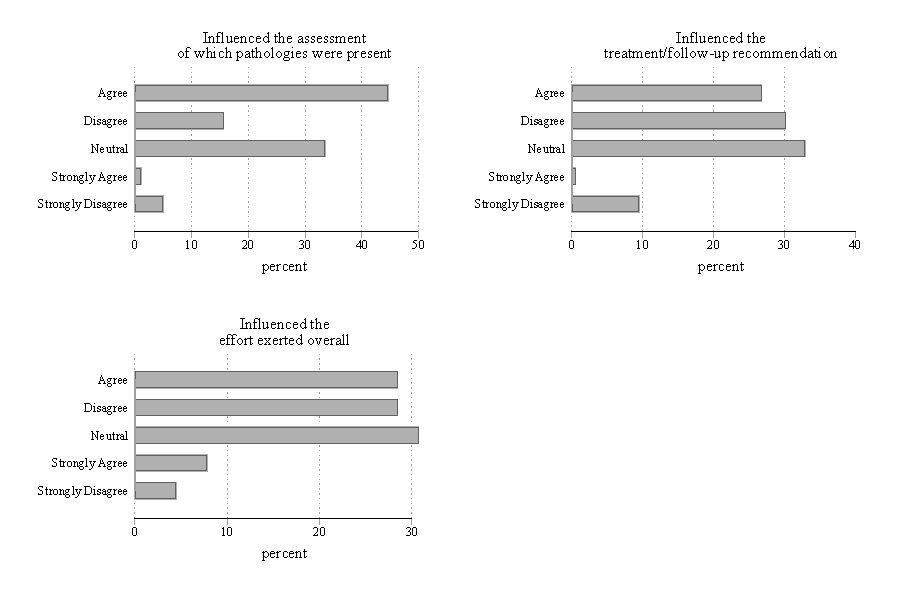
\includegraphics[width=0.8\textwidth]{ai_influence.pdf}
\end{center}
\end{figure}

Clinical history influence: Contrastingly, radiologists agreed to
the influence of clinical history on all three fronts of assessment,
decision-making and effort exertion. Clinical history is considered
to be a critical component in diagnostic radiology as it helps radiologists
to narrow down to specific regions in the X-ray. Concurrently, its
availability is believed to introduce cognitive biases like anchoring
bias, attribution bias and framing bias (Brennan and Ekpo). Given
these doubts about the benefits of clinical history, the radiologists'
probabilities and treatment decisions across different information
environments in the dataset can be uses to study its importance. Another
potential use of ththe quality of the clinical history indication
plays a huge role in ensuring an accurate diagnosis is that given
the varying levels of details in the clinical history indication available
to the radiologists, the importance of good quality clinical history
in decision accuracy can be studied. 

\begin{figure}[H]
\caption{Clinical History Influence\label{fig:ch-influence}}
\begin{center}
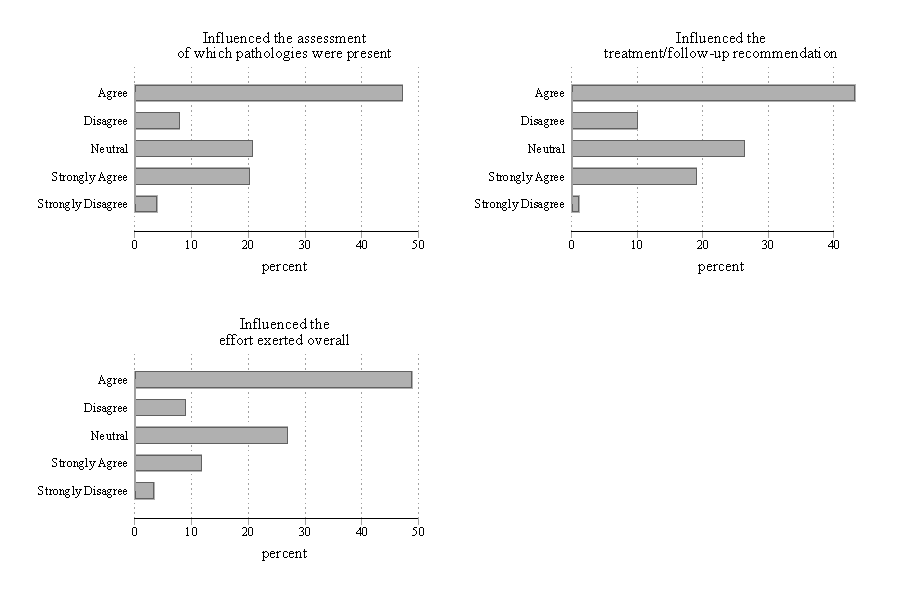
\includegraphics[width=0.8\textwidth]{ph_influence.pdf}
\end{center}
\end{figure}


\subsection*{Appendix: Variables \label{subsec:Appendix:-Variables} }

\begin{table}
\caption{Variable List}
%\begin{threeparttable}
\resizebox{\textwidth}{!}{%
\begin{tabular}{|l|l|l|l|}

\toprule[1pt]

Variable & Data Type & Range & Description \\
\hline
uid clean & str & & Radiologist identifier \\
design & dbl & ${1,2,3}$ & Design arm \\
patient id & str & & Patient identifier \\
pathology & str & & Pathology \\
round & long & $[1,100] \in N$ & Patient-case read sequence within radiologist-session \\
 & & & (minimum value is 1) \\
treat & int & ${0,1}$ & Indicator if radiologist selected treat/follow-up. \\
 & & &  Missing for pathologies where it was deemed not relevant \\
treatment & str & & Information environment under which case was read \\
level & int & ${0,1,2,3}$ & Position in pathology hierarchy (e.g. level 0 is top-level) \\
visible & int & ${0,1}$ & Indicator if pathology was visible when rad submitted case \\
probability & dbl & $[0,1]$ & Probability radiologist reported on interface slider \\
severity & str & & Response to severity question, when relevant \\
size & str & & Response to size question, when relevant\\
position & str & & Response to position question, when relevant \\
active time & dbl & & Time spent actively working on case (in seconds) \\
raw time & dbl & & Total time spent on case (in seconds) \\
num clicks & dbl & & Number of clicks on a case \\
group vietnam & int & ${0,1}$ & Indicator if the radiologist is from VinMac healthcare system, Vietnam \\
group teleradiology & int & ${0,1}$ & Indicator if the radiologist is from a tele radiology company \\
group pilot & int & ${0,1}$ & Indicator if the radiologist is from the experiment pilot \\
group ground truth & int & ${0,1}$ & Indicator if the radiologist is a ground truth radiologist \\
incentive round & int & ${0,1}$ & Indicator if incentives for correct diagnosis were provided \\
total num rounds & long & $[65,100]$ & The total number of reads by one radiologist  \\
chexbert label x & dbl & ${0,1}$ & ChexBert label for this case / pathology \\
ch indication & str & & Physician's indication for a given case \\
ch weight & str & & Weight(in lbs) of the patient under consideration \\
ch bp & str & & BP of the patient under consideration\\
ch temp & str & & Temperature of the patient under consideration \\
ch pulse & dbl & $[60,120]$ & Pulse of the patient under consideration \\
ch age & long & $[20,99]$ & Age of the patient under consideration \\
ch num labs & long & $[0,43]$ & Number of labels associated with a patient \\
ch num flagged labs & long & $[0,25]$ & Number of labels flagged as abnormal \\
ch gender & str & & Gender of the patient under consideration \\
alg pred & dbl & $[0,1]$ & AI prediction \\
with ai & byte & ${0,1}$ & Indicator if radiologist had access to AI \\
with ch & byte & ${0,1}$ & Indicator if radiologist had access to CH \\
gt average XX & dbl & $[0,1]$ & Average of ground truth probabilities for \\
 & & & group XX (us, vietnam, all, experiment) \\
gt average logodds XX & dbl & $[0,1]$ & Log-odds average (transformed into probability space) \\
 & & & probabilities for group XX \\
gt binary logodds XX & long & ${0,1}$ & Binary ground truth based on LO average for group XX \\
gt binary simple XX & long & ${0,1}$ & Binary ground truth based on simple average for group XX \\
gt treat XX & long & ${0,1}$ & Majority GT radiologists saying treat / follow-up for group XX \\
gt treat sum XX & dbl & ${0,1,2,3,4}$ & Number of GT radiologists saying treat / follow-up for group XX \\
gt average active time XX & dbl & $(35,344)$ & Average active time of the GT radiologists \\
ground truth & dbl & $[0,1]$ & Ground truth passed as an argument \\
ground truth treat & dbl & $[0,1]$ & Treatment ground truth, for group passed as argument \\
experiment id & str & & Radiologist identifier \\
experiment session & int & ${0,1,2,3}$ & Session number \\
case average active time & dbl & $[50,335]$ & Average time spent on a case by the radiologist \\
alg pred calibrated & dbl & $[0,1]$ & Calibrated version of the AI \\

\bottomrule[1pt]
\end{tabular}%
}
%\end{threeparttable}
\end{table}


\subsection*{Appendix: Experiment Interface \label{subsec:Appendix:-Experiment-Interface}}

The experimental interface was created with the intention to mimic
clinical practice while generating quantitative inputs for analysis.
Following is the information that the radiologists received before
starting the experiment. Comments on the instructions are provided
in italics and were not seen by subjects.

\subsubsection*{Section 1: Instructions}

You are about to participate in a study on medical decision making.
You may pause the study at any time. To resume, revisit the link you
were given and your progress will have been saved.

We will present you with adult patients with potential thoracic pathologies.
These patients will be presented under the following four scenarios:
\begin{enumerate}
\item Only a chest X-ray is shown.
\item An X-ray is accompanied with additional information about the \uline{clinical
history.}
\item An X-ray is shown along with \uline{Artificial Intelligence (AI)
support}. This AI tool is described in further detail below.
\item An X-ray is shown along with both additional information on \uline{clinical
history} and the \uline{AI support.}
\end{enumerate}
%
The patients are randomly assigned to each of these scenarios. That
is, availability of \uline{clinical history} and/or \uline{AI
support} is unrelated to the patient.

\uline{Clinical History:} includes available lab results or indications
by the treating physician, if any.

\uline{AI support:} This tool uses only the X-ray image to predict
the probability of each potential pathology of interest. The tool
is based on state-of-the-art machine learning algorithms developed
by a leading team of researchers at Stanford University.

\textbf{Responses}

For each patient and pathology, we will ask for both an assessment
and a treatment decision:
\begin{enumerate}
\item We will first ask for your assessment of the probability that each
condition is present in a patient. \textbf{Please consider all pathologies
and findings that would be relevant in a radiology report for the
patient. You should express your uncertainty about the presence of
one or many conditions by appropriately choosing the probability.}
Note that it is possible that the patient has multiple such conditions
or none of them.
\item If you determine that a pathology may be present, we may ask you to
rate the severity and/or extent of the disease on a scale.
\item Finally, when relevant we will ask whether you would recommend treatment
or follow up according to the clinical standard of care if you determine
that the pathology may be present. The first two responses are diagnostic
while the third is a clinical decision. We are aware that a single
physician or radiologist typically does not perform both tasks. However,
for this study, we ask that you respond to the best of your ability
in both of these roles.
\end{enumerate}
\textbf{Browser Compatibility}

This platform supports desktop versions of Chrome, Firefox, and Edge.
Important features on non-supported browsers (including Safari) are
missing and we discourage their use for this experiment. In addition,
the platform does not support any mobile devices and the platform
will perform poorly on mobile. If you encounter any issues during
the experiment, please send an email to \href{mailto:DiagnosticAI@mit.edu}{DiagnosticAI@mit.edu}
and we will follow-up quickly.

\subsubsection*{Section 2: Clinical Hierarchy}

The interface uses a hierarchy to categorize various thoracic conditions.
It will be useful to familiarize yourself with this hierarchy before
you start, but you may also revisit the hierarchy at any time throughout
the experiment by clicking the help tab in the upper right corner.\textit{
{[}The probability for the sub-pathologies is required only if the
parent pathology prevalence is greater than 10\%{]}}

\begin{figure}[H]
\caption{Pathology Hierarchy}

\begin{center}
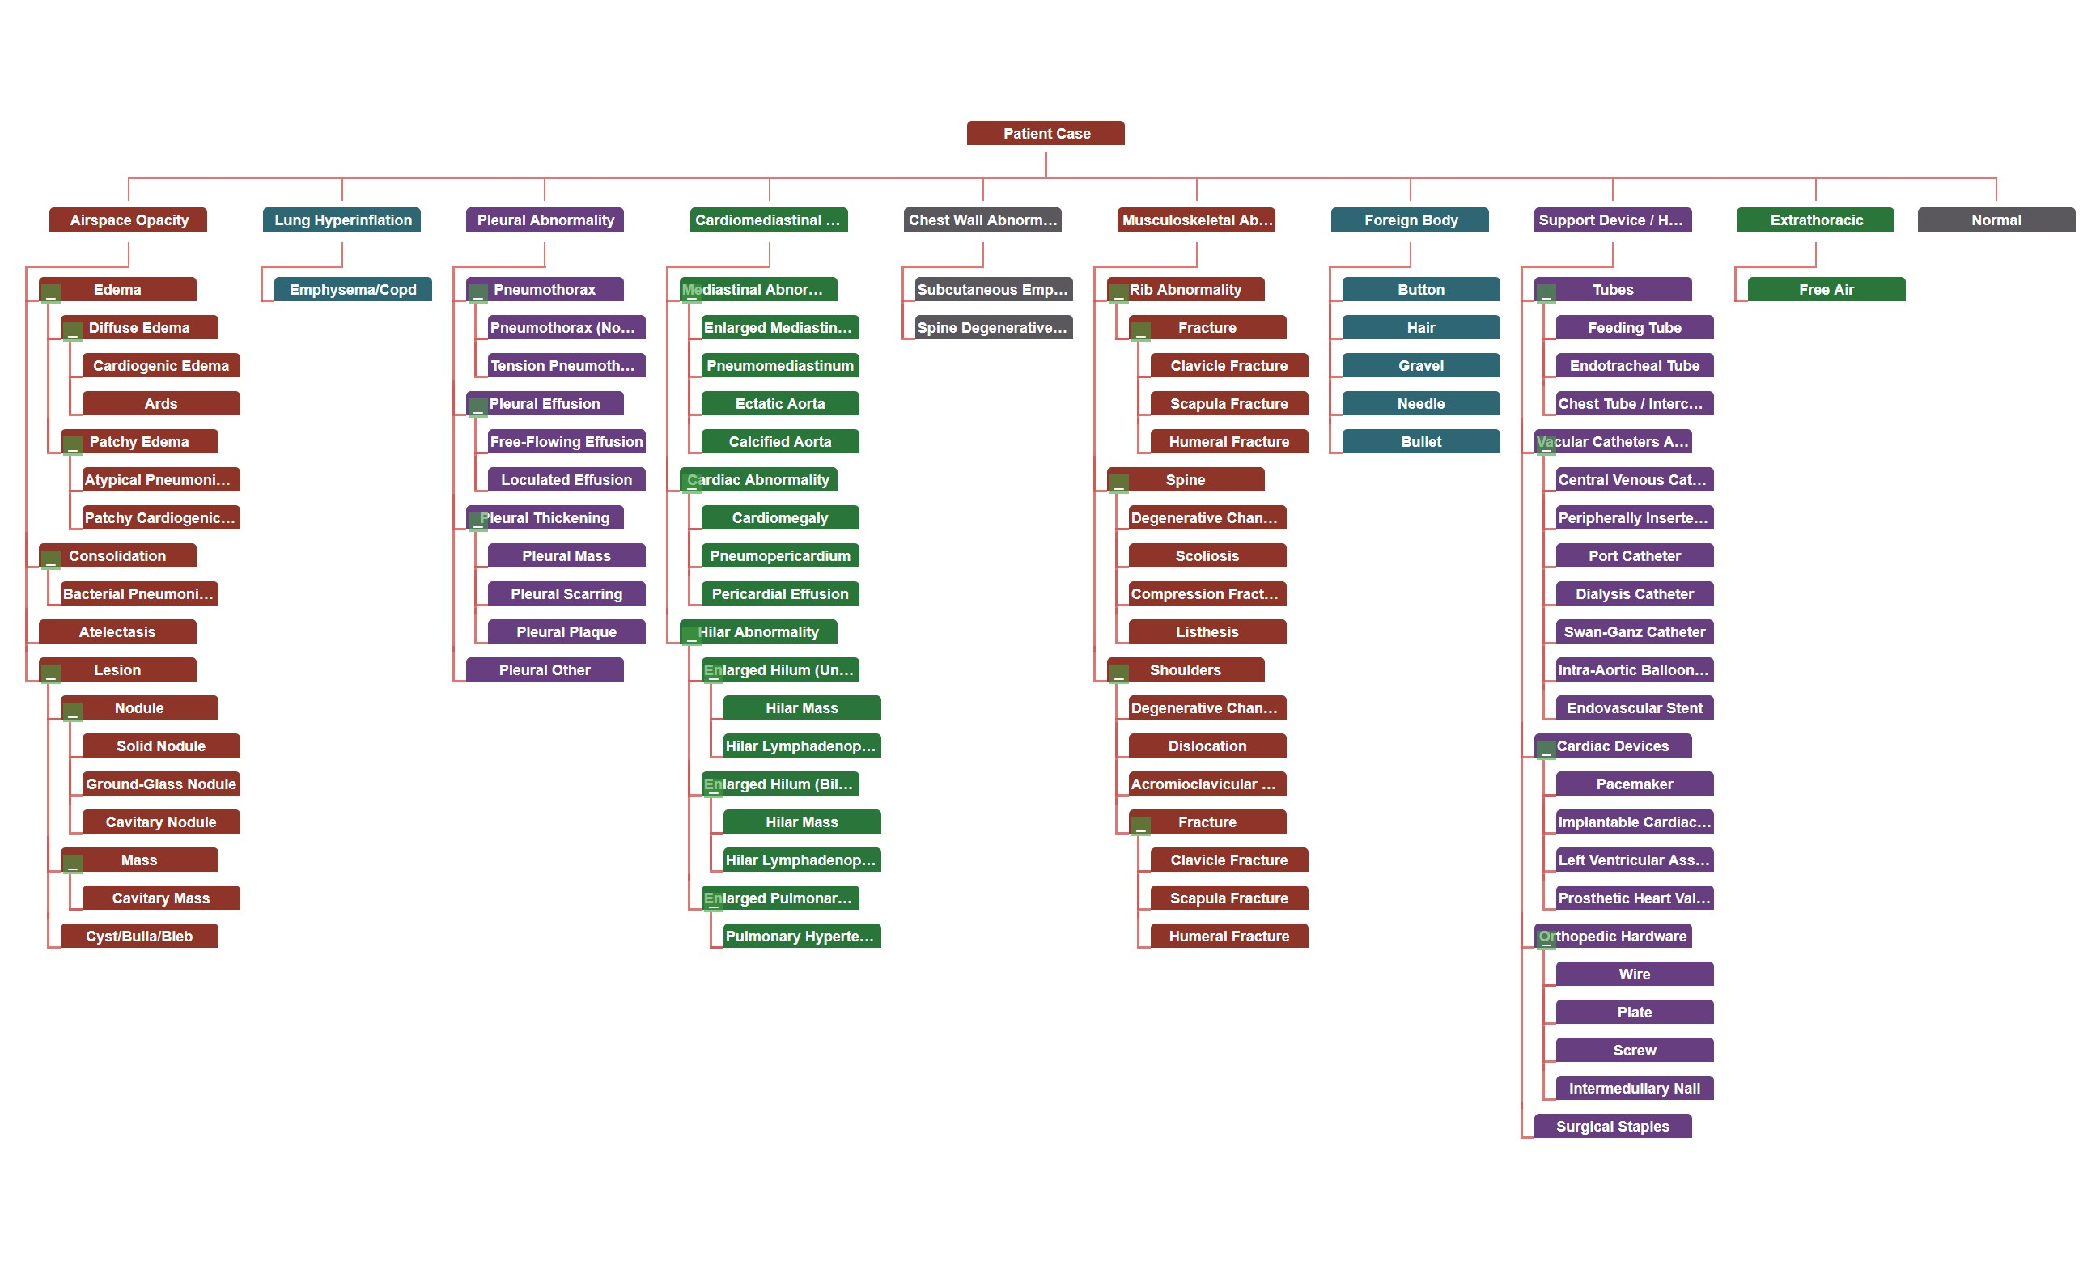
\includegraphics[width=1\textwidth]{images/pat_hierarchy.pdf}
\end{center}
\end{figure}


\subsubsection*{Section 3: AI Support Tool}

The AI support tool that is provided uses only the X-ray image to
predict the probability of each potential pathology of interest. The
tool is based on state-of-the-art machine learning algorithms developed
by a leading team of researchers at Stanford University. The tool
is trained only on X-ray images, meaning it does not incorporate the
clinical history of the patients.

\textbf{Performance of the AI Support}

The AI tool is described in \href{https://arxiv.org/abs/1901.07031}{Irvin et al. [2019]},
which showed the AI tool performed at or near expert levels across
the pathologies studied. Below we plot two measures of performance
of the AI tool. We plot in blue the accuracy of the tool, defined
as the share of cases correctly diagnosed when treating false positives
and false negatives equally. In red, we plot the Area Under the ROC
curve (AUC), which is another measure of AI classification performance.
The AUC is a number between 0 and 100\%, with numbers close to 100\%
representing better algorithm performance. The AUC is equal to the
probability that a randomly chosen positive case is ranked higher
than a randomly chosen negative case.

\begin{figure}[H]
\caption{Performance of AI Tool}

\begin{center}
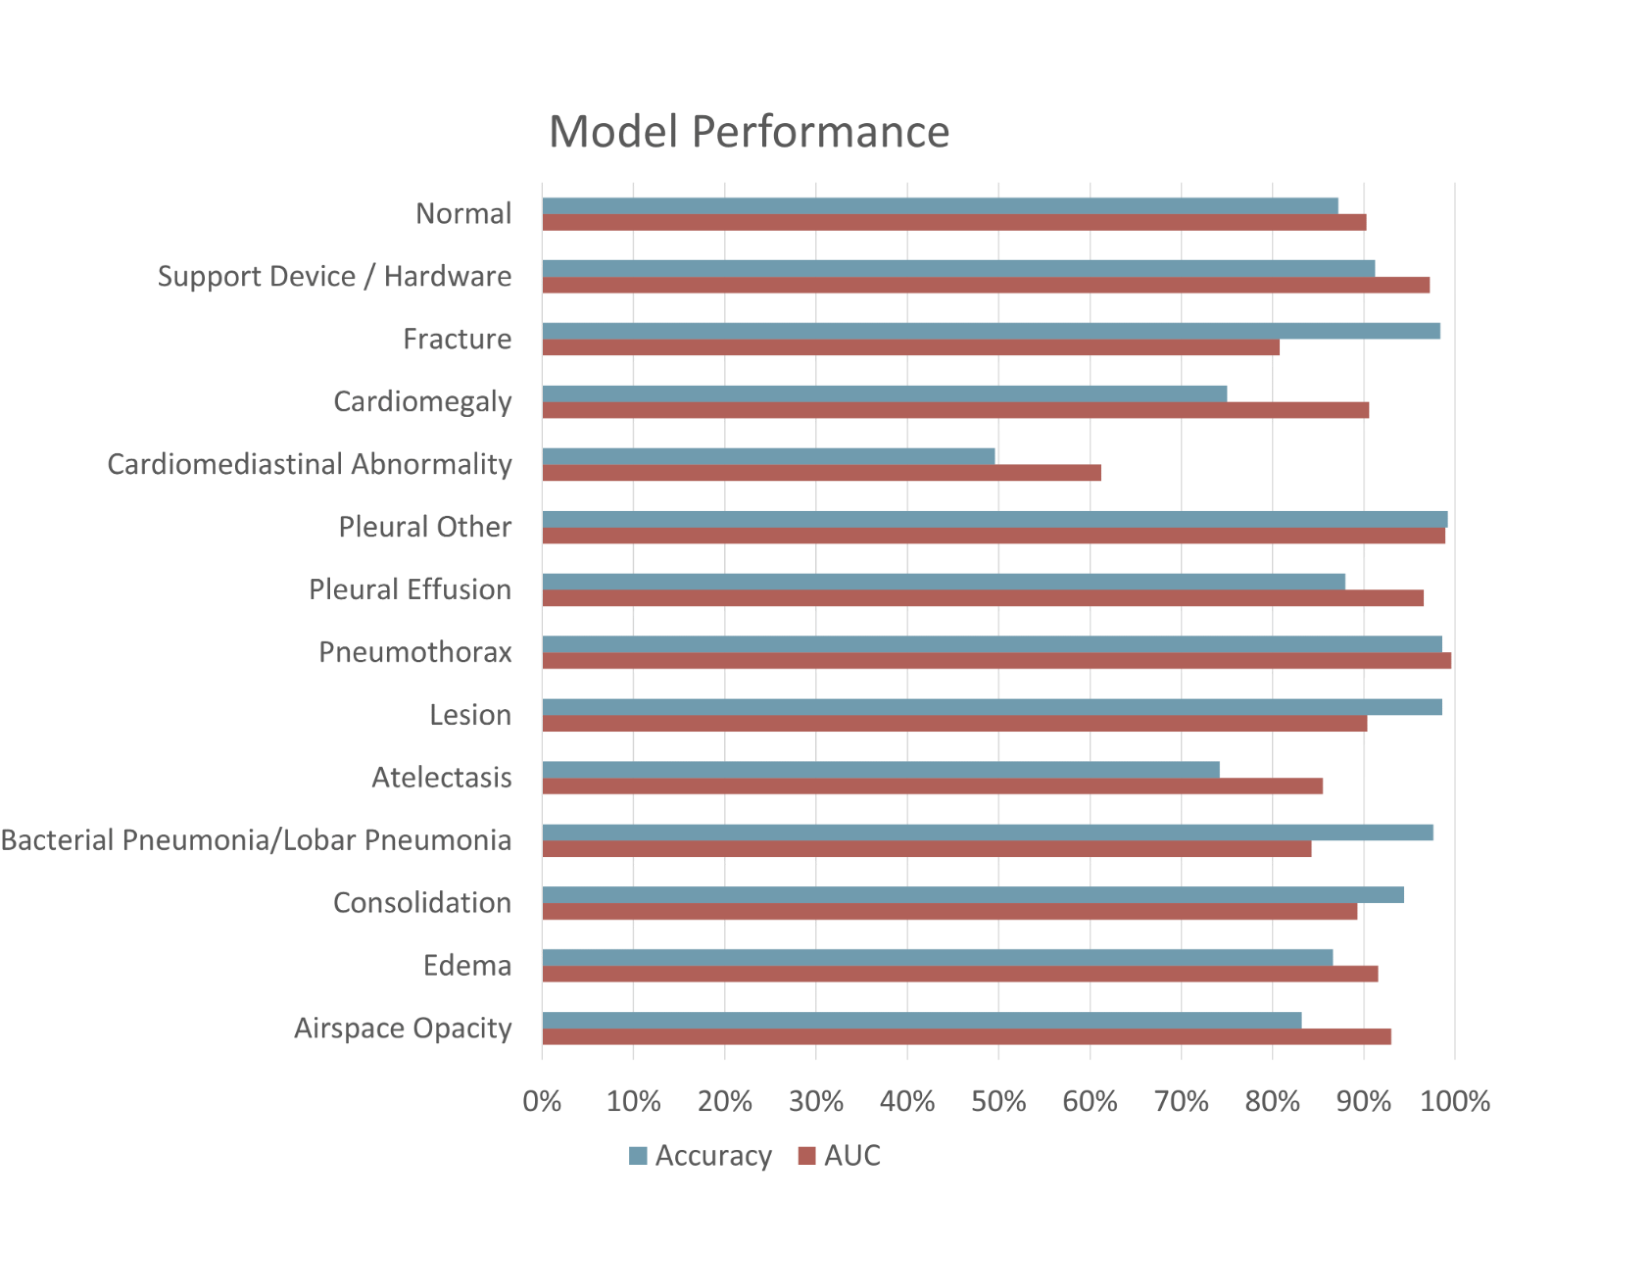
\includegraphics[scale=0.6]{images/ai_instruction_accuracy.pdf}
\end{center}
\end{figure}

\textbf{Example Images}

Below are 50 example images with the associated AI tool predictions.
These images are randomly chosen to allow you to familiarize yourself
with the AI support tool and its accuracy \emph{{[}Here we only provide
two out of the fifty images{]}.}

\begin{figure}[H]
\caption{Example Images}

\begin{center}
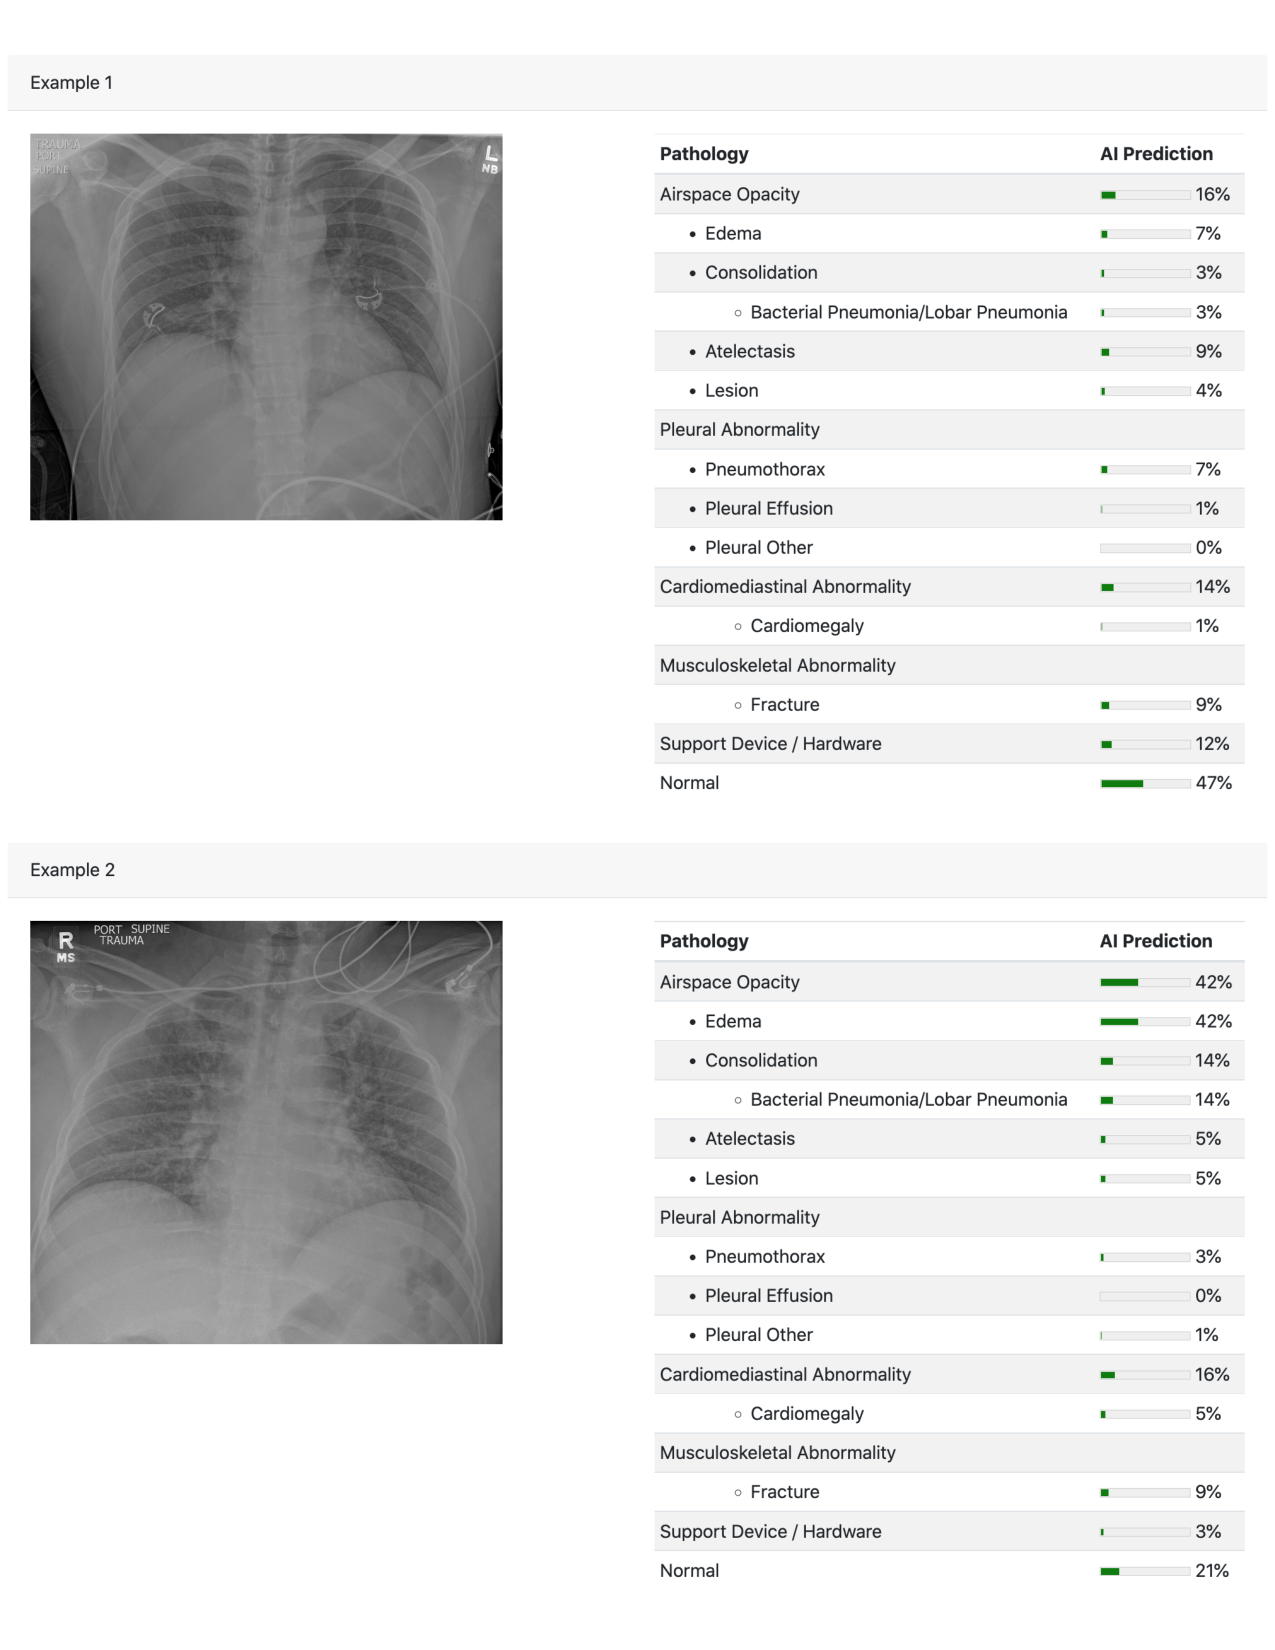
\includegraphics[scale=0.8]{images/ai_instruction_example.pdf}
\end{center}
\end{figure}
\textbf{Section 4: Demonstration}

The brief video below walks you through the interface and a few examples.
\emph{{[}At this stage participants saw an instruction video which
can be founds \href{https://www.dropbox.com/s/fgdcokweekpm44r/RadExperimentV4.mp4?raw=1}{here}{]}}

\subsubsection*{Section 5: Consent I}

You have been asked to participate in a study conducted by researchers
from the Massachusetts Institute of Technology (M.I.T.) and Harvard
University.

The information below provides a summary of the research. Your participation
in this research is voluntary and you can withdraw at any time.
\begin{enumerate}
\item Study procedure: We will ask you to examine a number of chest x-rays.
We will vary both the amount of information provided about the patient
and the availability of an AI support tool.
\item Potential Risks \& Benefits: There are no foreseeable risks associated
with this study and you will receive no direct benefit from participating.
\end{enumerate}
%
Your participation in this study is completely voluntary and you are
free to choose whether to be in it or not. If you choose to be in
this study, you may subsequently withdraw from it at any time without
penalty or consequences of any kind. The investigator may withdraw
you from this research if circumstances arise.

\subsubsection*{Section 6: Consent II}

\textbf{Privacy \& Confidentiality}

The only people who will know that you are a research subject are
members of the research team which might include outside collaborators
not affiliated with MIT. No identifiable information about you, or
provided by you during the research, will be disclosed to others without
your written permission, except: if necessary to protect your rights
or welfare, or if required by law. In addition, your information may
be reviewed by authorized MIT representatives to ensure compliance
with MIT policies and procedures.

When the results of the research are published or discussed in conferences,
no information will be included that would reveal your identity.

\textbf{Questions}

If you have any questions or concerns about the research, please feel
free to contact us directly at diagnosticAI@mit.edu.

\textbf{Your Rights}

You are not waiving any legal claims, rights or remedies because of
your participation in this research study. If you feel you have been
treated unfairly, or you have questions regarding your rights as a
research subject, you may contact the Chairman of the Committee on
the Use of Humans as Experimental Subjects, M.I.T., Room E25-143B,
77 Massachusetts Ave, Cambridge, MA 02139, phone 1-617-253 6787.

I understand the procedures described above. By clicking next, I am
acknowledging my questions have been answered to my satisfaction,
and I agree to participate in this study.

\subsubsection*{Section 7: Interface questions}

\emph{{[}Each of these questions has a true of false response which
was entered through a radio button. Participants are not able to start
the experiment without answering each question correctly.{]}}

Before beginning the experiment, we would like to confirm a few facts
through the following comprehension questions. Please answer True
or False to the following questions.

1) The algorithm's prediction is based on information from both the
X-ray scan as well as the clinical history.

2) When the algorithm does not show a prediction, it is because the
algorithm thinks the pathology is not present.

3) The follow up decision refers to any treatment or additional diagnostic
procedures that one would conduct based on the findings of the report.

4) Two patients with the same probability score for a condition ought
to always receive the same \textquotedblleft follow-up\textquotedblright{}
recommendation.

5) When a condition at a higher level of the hierarchy receives a
less than ten percent chance of being present then all the lower level
conditions within this branch automatically receive a zero probability
of being present.

6) If the algorithm says that the probability of a pathology is present
with 80\% probability, it means that the AI predicts 80 cases out
of 100 have the pathology present.

7) Suppose your assessment is that the patient definitely has either
edema or consolidation, and you believe that edema is twice as likely
as consolidation. Then you would assign 66.67\% to edema and 33.33\%
to consolidation:

8) I should only indicate pathologies and findings that would be relevant
in a radiology report for the patient.

\subsubsection*{Section 8: Bonus (Randomized only for designs 1 and 3)}

Bonus Payment Thank you again for participating in our study. If your
responses in this section are close to the average response of an
independent group of radiologists for each case, we will give you
a \$120 gift card to a large e-commerce retailer of your choice (e.g.
Amazon, Flipkart). This payment rule is designed so that your chances
of winning the prize is highest if you report your best estimate of
the probability that the pathology is present. The precise payment
rule is available on request, and we will follow up after the experiment
if you win the gift card.

\subsubsection*{Section 9: Practice Images}

First, we will present you with 8 patients (Design 1) to practice
and familiarize yourself with the interface. In the practice you will
see 2 patient cases under each of the possible combinations of AI
support and clinical history availability. You will be compensated
for these reads even though they are just for practice. {[}\textit{5
practice images for design 1 and none for design 3}{]}

\subsubsection*{Section 10: Randomized Information Scenario }

{[}\textit{This is the start of the experiment. The dataset contains
only these observations and excludes any practice images data.}{]}

The extent of clinical history information provided is not homogenous.
The thoroughness of the information varies across available information
for every patient. Some examples of varying clinical history information
are: 



\end{document}
